\section{Pre-Processing}
\label{sec:ImPros}
Before the classifiers will be trained, some pre-processing is needed. In order to make all images the same size, they were placed within the same bounding box. Next, all images were downsampled to a size of 16 by 16 pixels, to reduce the amount of pixels and save computational time and space. \\
Then some image processing was implemented. When looking at some random samples of the dataset, it was noticed that some of them contained fragmented digits. Also, some spots and blobs could be observed in some images. When using certain Pattern Recognition tools, this could create various problems. For instance, when using a feature-representation to classify the objects, the feature 'perimeter' will look for the first object in every image, and calculate its perimeter. If a small blob is present in the top left corner of an image, it will calculate the perimeter of this blob, and ignore the actual digit. \\
In order to overcome this problem relatively easy, two image processing steps are implemented in the pre-processing phase. First, all images were extracted from the dataset and converted to an image using the \texttt{data2im.m} in MatLab. This means that all kinds of image-processing techniques become available. Since this course focusses on Pattern Recognition, and not so much on Image Processing, it was decided to keep it relatively simple, and just implement two functions to remove some of the spots and blobs. \texttt{bwmorph.m} was used to remove single pixels, and \texttt{bwareaopen.m} was used to remove some larger blobs. After this, the images were converted back to data using \texttt{im2obj.m}, and stored in a prdataset. \\
Finally, a small gaussian filter was used to overcome some 'broken' digits and smooth out some rough edges that originated from the downsampling. While more advanced techniques like image propagation would be more suitable to close for instance sixes and eights, it was decided not to implement this in the interest of time and with the goal of the course in mind. A few examples the pre-processing has on some digits can be seen in figure \ref{fig:Image_Prepros}.
\begin{figure}[H]
	\centering
	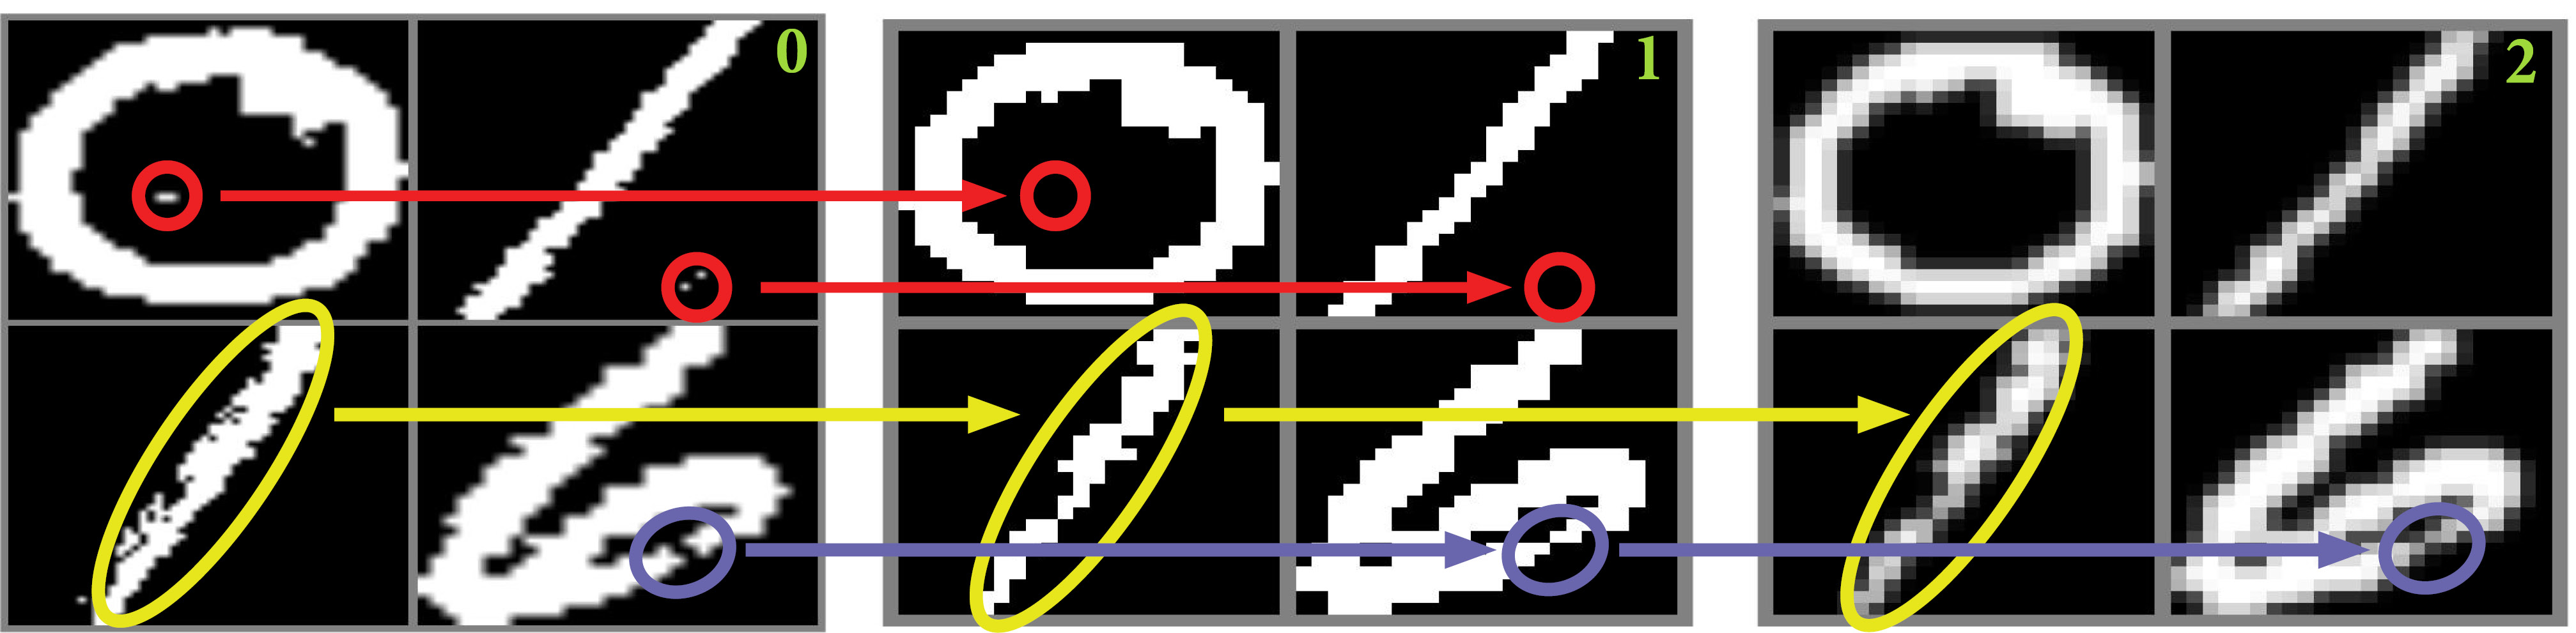
\includegraphics[scale=0.45]{images/Image_Prepros.jpg}
	\caption{Effect the pre-processing has on certain defects in the images. Step 1 removes single pixels and small blobs using \texttt{bwmorph.m} and \texttt{bwareaopen.m}. Step 2 adds a gaussian filter, to reconnect broken digits and smooth out any rough edges.}
	\label{fig:Image_Prepros}
\end{figure}